\documentclass[12pt,letterpaper]{article}

\newenvironment{proof}{\noindent{\bf Proof:}}{\qed\bigskip}

\newtheorem{theorem}{Theorem}
\newtheorem{corollary}{Corollary}
\newtheorem{lemma}{Lemma} 
\newtheorem{claim}{Claim}
\newtheorem{fact}{Fact}
\newtheorem{definition}{Definition}
\newtheorem{assumption}{Assumption}
\newtheorem{observation}{Observation}
\newtheorem{example}{Example}
\newcommand{\qed}{\rule{7pt}{7pt}}

\newcommand{\assignment}[4]{
\thispagestyle{plain} 
\newpage
\setcounter{page}{1}
\noindent
\begin{center}
\framebox{ \vbox{ \hbox to 6.28in
{\bf CS440: Introduction to Artificial Intelligence \hfill #1}
\vspace{4mm}
\hbox to 6.28in
{\hspace{2.5in}\large\mbox{In class assignment #2}}
\vspace{4mm}
\hbox to 6.28in
{{\it Handed Out: #3 \hfill Due: #4}}
}}
\end{center}
}

\newcommand{\solution}[4]{
\thispagestyle{plain} 
\newpage
\setcounter{page}{1}
\noindent
\begin{center}
\framebox{ \vbox{ \hbox to 6.28in
{\bf CS440 : Introduction to Artificial Intelligence \hfill #4}
\vspace{4mm}
\hbox to 6.28in
{\hspace{2.5in}\large\mbox{In class assignment #3}}
\vspace{4mm}
\hbox to 6.28in
{#1 \hfill {\it Handed In: #2}}
}}
\end{center}
\markright{#1}
}

\newenvironment{algorithm}
{\begin{center}
\begin{tabular}{|l|}
\hline
\begin{minipage}{1in}
\begin{tabbing}
\quad\=\qquad\=\qquad\=\qquad\=\qquad\=\qquad\=\qquad\=\kill}
{\end{tabbing}
\end{minipage} \\
\hline
\end{tabular}
\end{center}}

\def\Comment#1{\textsf{\textsl{$\langle\!\langle$#1\/$\rangle\!\rangle$}}}


\usepackage{algorithm}
\usepackage{listings}
%\usepackage{algpseudocode}
\usepackage{graphicx,amssymb,amsmath}
\usepackage{epstopdf}
\usepackage{color}
\usepackage{listings}
\lstset{ %
language=Java,                % choose the language of the code
basicstyle=\footnotesize,       % the size of the fonts that are used for the code
numbers=left,                   % where to put the line-numbers
numberstyle=\footnotesize,      % the size of the fonts that are used for the line-numbers
stepnumber=1,                   % the step between two line-numbers. If it is 1 each line will be numbered
numbersep=5pt,                  % how far the line-numbers are from the code
backgroundcolor=\color{white},  % choose the background color. You must add \usepackage{color}
showspaces=false,               % show spaces adding particular underscores
showstringspaces=false,         % underline spaces within strings
showtabs=false,                 % show tabs within strings adding particular underscores
frame=single,           % adds a frame around the code
tabsize=2,          % sets default tabsize to 2 spaces
captionpos=b,           % sets the caption-position to bottom
breaklines=true,        % sets automatic line breaking
breakatwhitespace=false,    % sets if automatic breaks should only happen at whitespace
escapeinside={\%*}{*)}          % if you want to add a comment within your code
}
\sloppy


\oddsidemargin 0in
\evensidemargin 0in
\textwidth 6.5in
\topmargin -0.5in
\textheight 9.0in

\begin{document}

\solution{Dan McQuillan}{\today}{4 - Problem 1}{Spring 2014}

\pagestyle{myheadings}  % Leave this command alone

\begin{enumerate}

	\item {\bf Problem 1 - General Classification}
	
		\begin{enumerate}
		
			\item[(a)] 
				
				\begin{enumerate}
				
					\item[(i)]
					For each \(N = \left\{ 10, 30, 50, 70, 90 \right\} \) report the accuracy of the classifier over the training data and the accuracy over the testing data.
					
					\[
						\begin{array}{c|cc}
							N & \text{Training Accuracy} & \text{Testing Accuracy} \\
							\hline
							10 & 100.0 & 61.21495327102804 \\
							30 & 87.5 & 68.22429906542057 \\
							50 & 85.04672897196262 & 74.29906542056075 \\
							70 & 83.89261744966443 & 78.03738317757009 \\
							90 & 85.41666666666667 & 83.64485981308411 \\
						\end{array}
					\]
					
					\item[(ii)] Plot accuracy on training data vs. N and accuracy on testing data vs. N on the same plot
					
						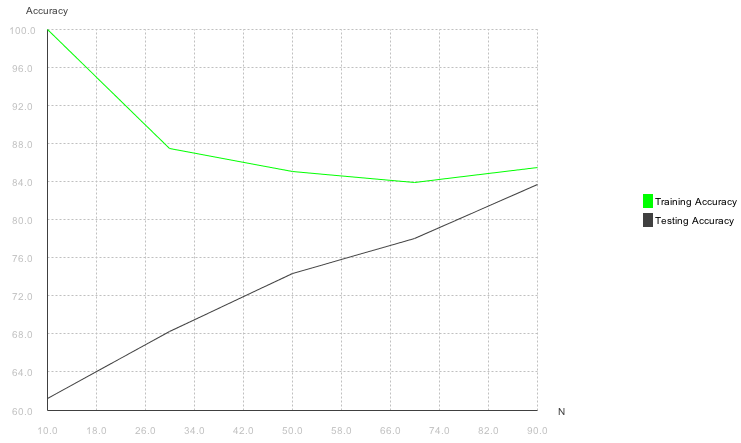
\includegraphics[scale=0.5]{p1a-ii-graph}
										
					\item[(iii)] Explain the results
					
						The result is as expected since with each value of N the amount of training examples is increasing. Therefore, with each next value of N the accuracy will also increase since the bias is increasing.  However, since the number of epochs in the weka implementation is constrained to 500 the classifier may not always converge which explains why the accuracy of the classifier drops when more samples are used.
						
				\end{enumerate}
			
			\item[(b)] 
				
					\[
						\begin{array}{c|ccc}
							N & \text{Time Taken} & \text{Percent Correct} & \text{Percent Incorrect} \\
							\hline
							2 & 0.621s & 63.08411214953271 & 36.91588785046729 \\
							5 & 1.947s & 60.2803738317757 & 39.7196261682243 \\
							10 & 4.276s & 66.35514018691589 & 33.64485981308411 \\
							15 & 6.571s & 68.22429906542057 & 31.77570093457944 \\
							20 & 9.0s & 66.82242990654206 & 33.177570093457945 \\
						\end{array}
					\]
					
				\begin{enumerate}
				
					\item[(i)] Plot the accuracy vs. n
					
						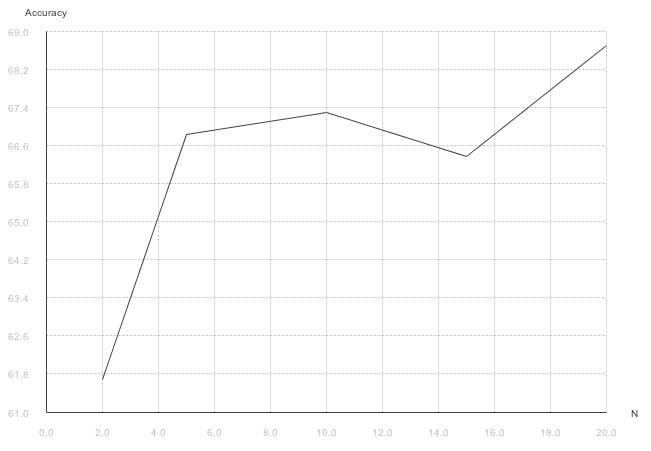
\includegraphics[scale=0.5]{p1b-i-graph}
					
					\item[(ii)] Plot the time taken by cross validation vs. n
					
						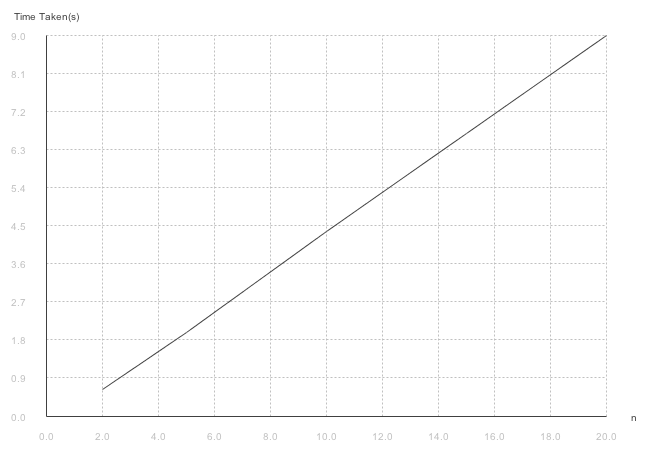
\includegraphics[scale=0.5]{p1b-ii-graph}
					
					\item[(iii)] Discuss the advantages of using n-fold cross validation as opposed to the testing method we used in part a \\
					
					The advantage of using n-fold cross validation is simply that the learning of which partitions of data to be used is also learned by k-fold cross validation.  Also this not only constrains the data but also randomizes the partitions of the selected data to the optimal partitions for the classifier.
					
					\item[(iv)] Discuss the advantages and disadvantages of using a large n \\
					
					The advantages of using a large n is you will get a set of partitions with smaller size and therefore the resultant classifier will use a larger set of data when it has finished and will eliminate a lot of the invalid priori.  However the disadvantage comes with the processing time of the cross validation as shown in the graph from part b.ii.
					
					
				\end{enumerate}
						
		\end{enumerate}	 	

\end{enumerate}

\section{Source Code:}

\subsection{ClassifierWrapper.java}

\begin{lstlisting}
package hw4.weka;

public class ClassifierWrapper {
	
	private Double trainingAccuracy;
	private Double testingAccuracy;
	private final MultilayerPerceptronClassifier classifier;
	
	public ClassifierWrapper( final Double trainingAccuracy, final Double testingAccuracy, final MultilayerPerceptronClassifier classifier ) {
		this.trainingAccuracy = trainingAccuracy;
		this.testingAccuracy = testingAccuracy;
		this.classifier = classifier;
	}

	public Double getTrainingAccuracy() {
		return trainingAccuracy;
	}

	public Double getTestingAccuracy() {
		return testingAccuracy;
	}

	public MultilayerPerceptronClassifier getClassifier() {
		return classifier;
	}
	
	public void setTrainingAccuracy(Double trainingAccuracy) {
		this.trainingAccuracy = trainingAccuracy;
	}

	public void setTestingAccuracy(Double testingAccuracy) {
		this.testingAccuracy = testingAccuracy;
	}

	@Override
	public String toString() {
		StringBuilder stringBuilder = new StringBuilder();
		stringBuilder.append("Training Accuracy: " + trainingAccuracy );
		stringBuilder.append("\n");
		stringBuilder.append("Testing Accuracy: " + testingAccuracy );
		stringBuilder.append("\n");
		
		return stringBuilder.toString();
	}

}
\end{lstlisting}

\subsection{MultilayerPerceptronClassifier.java}

\begin{lstlisting}
package hw4.weka;

import weka.classifiers.functions.MultilayerPerceptron;
import weka.core.Instances;

public class MultilayerPerceptronClassifier {

	private Instances instances = null;
	
	private Double N = 0.0;
	
	private MultilayerPerceptron percep;
	
	public MultilayerPerceptronClassifier( final Instances instances, final Double N ) {
		this.instances = instances;
		this.N = N;
	}
	
	public Double classify() throws Exception {
		int numInstances = instances.numInstances();

		instances.setClassIndex(instances.numAttributes() - 1);
		
		percep = new MultilayerPerceptron();
		Instances trainingData = new Instances(instances, 0, (int) (numInstances * (N  / 100.0 )) );
		
		percep.buildClassifier(trainingData);
		
		return test(instances, N );

	}
	
	public Double test(Instances testingInstances, Double N ) throws Exception {
		int numInstances = testingInstances.numInstances();
		
		Instances testingData = new Instances(
				instances,
				0,
				(int) (numInstances * (N  / 100.0 ))
			);

		double correct = 0.0;
		double incorrect = 0.0;
		
		for( int i = 0; i < testingData.numInstances(); i++) {
			double assignedClass = percep.classifyInstance(testingData.instance(i));
			double originalClass = testingData.instance(i).classValue();
			
			if( assignedClass == originalClass ) {
				correct++;
			} else {
				incorrect++;
			}
		}
		
		Double accuracy = 100.0 * correct / (correct + incorrect);
		
		return accuracy;
	}
}
\end{lstlisting}

\subsection{Pair.java}

\begin{lstlisting}
package hw4.weka;

public class Pair<T, V> {

	T left;
	V right;
	
	public T getLeft() {
		return left;
	}
	public void setLeft(T left) {
		this.left = left;
	}
	public V getRight() {
		return right;
	}
	public void setRight(V right) {
		this.right = right;
	}
	
	
}
\end{lstlisting}

\subsection{Tuple3.java}

\begin{lstlisting}
package hw4.weka;

public class Tuple3<T, V, W> {

	T first;
	V second;
	W third;
	
	public T getFirst() {
		return first;
	}
	public void setFirst(T first) {
		this.first = first;
	}
	public V getSecond() {
		return second;
	}
	public void setSecond(V second) {
		this.second = second;
	}
	public W getThird() {
		return third;
	}
	public void setThird(W third) {
		this.third = third;
	}	
}
\end{lstlisting}

\subsection{Main.java}

\begin{lstlisting}
package hw4.weka;

import java.awt.Color;
import java.io.BufferedReader;
import java.io.BufferedWriter;
import java.io.File;
import java.io.FileReader;
import java.io.FileWriter;
import java.io.IOException;
import java.util.ArrayList;
import java.util.Collections;
import java.util.Date;
import java.util.HashMap;
import java.util.List;
import java.util.Map;
import java.util.Random;

import javax.swing.JFrame;

import org.math.plot.Plot2DPanel;

import weka.classifiers.evaluation.Evaluation;
import weka.classifiers.evaluation.output.prediction.XML;
import weka.classifiers.functions.MultilayerPerceptron;
import weka.core.Instances;

public class Main {

	public static void main(String[] args) {

		try {
			File file = new File("data/glass.arff");
			BufferedReader bufferedReader = new BufferedReader(new FileReader(file));
			
			Instances instances = new Instances(bufferedReader);
			
			bufferedReader.close();
			
			StringBuilder applicationOutput = new StringBuilder();
			applicationOutput.append("**************************\n").append("**************************\n").append("**************************\n")
							 .append("Begin Part A\n")
							 .append("**************************\n").append("**************************\n").append("**************************\n");
			// Part a
			double[] nValues = new double[] { 
					10.0,
					30.0,
					50.0,
					70.0,
					90.0
			};
			
			Map<Double, ClassifierWrapper> classificationResults = new HashMap<Double, ClassifierWrapper>();
			double accuracyArray[] = new double[5];
			double trainingAccuracyArray[] = new double[5];
			int i = 0;
			for( Double N : nValues ) {
				
				ClassifierWrapper wrapper = new ClassifierWrapper(
						null,
						null,
						new MultilayerPerceptronClassifier(instances, N)
					);
				
				wrapper.setTrainingAccuracy( wrapper.getClassifier().classify() );
				wrapper.setTestingAccuracy( wrapper.getClassifier().test( instances, 100.0 ) );
				classificationResults.put( N, wrapper );

				trainingAccuracyArray[i] = wrapper.getTrainingAccuracy();
				accuracyArray[i++] = wrapper.getTestingAccuracy();
				
				applicationOutput.append( wrapper.toString() ).append("\n");
			}	
			
//			Plot2DPanel plot = new Plot2DPanel();
//			plot.addLinePlot("Training Accuracy", Color.GREEN, nValues, trainingAccuracyArray);
//			plot.addLinePlot("Testing Accuracy", Color.darkGray, nValues, accuracyArray);
//			plot.setLegendOrientation("NORTH");
//			JFrame frame = new JFrame("Problem 1a Results");
//			plot.setAxisLabels(new String[] { "N", "Accuracy" });
//			frame.setContentPane(plot);
//			frame.setVisible(true);
//			frame.setSize(800, 600);
						
			applicationOutput.append("**************************\n").append("**************************\n").append("**************************\n")
							 .append("End Part A\n")
							 .append("**************************\n").append("**************************\n").append("**************************\n\n");
			
			applicationOutput.append("**************************\n").append("**************************\n").append("**************************\n")
							 .append("Begin Part B\n")
							 .append("**************************\n").append("**************************\n").append("**************************\n");
							
			// Part b			
			int[] foldsArray = new int[] {
					2,
					5,
					10,
					15,
					20
			};
			
			double[] foldsDoubleArray = new double[] {
					2,
					5,
					10,
					15,
					20
			};
			
			Instances trainInstances = instances;
			Map<Integer, Tuple3<StringBuffer, Evaluation, Double>> results = new HashMap<Integer, Tuple3<StringBuffer, Evaluation, Double>>();
			for( final Integer folds : foldsArray ) {
				Tuple3<StringBuffer, Evaluation, Double> tuple3 = new Tuple3<StringBuffer, Evaluation, Double>();
				
				StringBuffer internalStringBuffer = new StringBuffer();
				XML internalOutput = new XML();
				internalOutput.setBuffer(internalStringBuffer);
				internalOutput.setHeader(trainInstances);
				internalOutput.setOutputDistribution(true);

				Evaluation evaluation = new Evaluation(trainInstances);
				
				MultilayerPerceptron percep = new MultilayerPerceptron();
				Date beforeCrossValidate = new Date();
				evaluation.crossValidateModel(percep, trainInstances, folds, new Random( new Date().getTime() ), internalOutput );
				Date afterCrossValidate = new Date();
				
				Double timeTakenCrossValidation =  ((double)( afterCrossValidate.getTime() - beforeCrossValidate.getTime())) / 1000.0;
				
				tuple3.setFirst( internalStringBuffer );
				tuple3.setSecond( evaluation );
				tuple3.setThird( timeTakenCrossValidation );
				
				results.put(folds, tuple3);
			}
			List<Integer> keySet = new ArrayList<Integer>();
			for( Integer key : results.keySet() ) {
				keySet.add(key);
			}
			Collections.sort(keySet);
			accuracyArray = new double[5];
			double timeTakenArray[] = new double[5];
			i = 0;
			for( final Integer key : keySet ) {
				Tuple3<StringBuffer, Evaluation, Double> result = results.get(key);
				File outputFile = new File("result/cross-validation-output-" + key + ".xml");
				if( outputFile.exists() ) {
					outputFile.delete();
				}
				
				BufferedWriter bufferedWriter = new BufferedWriter(new FileWriter(outputFile));
				bufferedWriter.write(result.getFirst().toString());
				bufferedWriter.close();
				
				timeTakenArray[i] = result.getThird();
				accuracyArray[i++] = result.getSecond().pctCorrect();
				
				applicationOutput.append("***********************************\nCross Validation Result\n***********************************\n");
				applicationOutput.append("Results for N = ").append(key).append("\n");
				applicationOutput.append("Time taken: " + result.getThird() + "s\n");
				applicationOutput.append("Percent Correct: " + result.getSecond().pctCorrect() + "\n");
				applicationOutput.append("Percent Incorrect: " + result.getSecond().pctIncorrect() + "\n");
				applicationOutput.append("Confusion Matrix: \n" + result.getSecond().confusionMatrix() + "\n\n");
//				applicationOutput.append("------------\nXML Data\n------------\n\n").append( result.getFirst().toString() ).append("\n\n");
			}
			
			Plot2DPanel plot2 = new Plot2DPanel();
			plot2.addLinePlot("n vs. Accuracy", Color.DARK_GRAY, foldsDoubleArray, accuracyArray);
			JFrame frame2 = new JFrame("Problem 1b Results");
			plot2.setAxisLabels(new String[] { "N", "Accuracy" });
			frame2.setContentPane(plot2);
			frame2.setVisible(true);
			frame2.setSize(800, 600);

			
			Plot2DPanel plot3 = new Plot2DPanel();
			plot3.addLinePlot("n vs. Time Taken by Cross Validation", Color.DARK_GRAY, foldsDoubleArray, timeTakenArray);
			JFrame frame3 = new JFrame("Problem 1b Results");
			plot3.setAxisLabels(new String[] { "n", "Time Taken(s)" });
			frame3.setContentPane(plot3);
			frame3.setVisible(true);
			frame3.setSize(800, 600);
			
			applicationOutput.append("**************************\n").append("**************************\n").append("**************************\n")
							 .append("End Part B\n")
							 .append("**************************\n").append("**************************\n").append("**************************\n");
		
			System.out.println(applicationOutput.toString());
		} catch (IOException e) {
			System.err.println( e );
		} catch (Exception e) {
			e.printStackTrace();
		}
		
	}

}
\end{lstlisting}
\end{document}

